% Figures for 147 Atoms 
\begin{figure}[!h] 
    \begin{center} 
        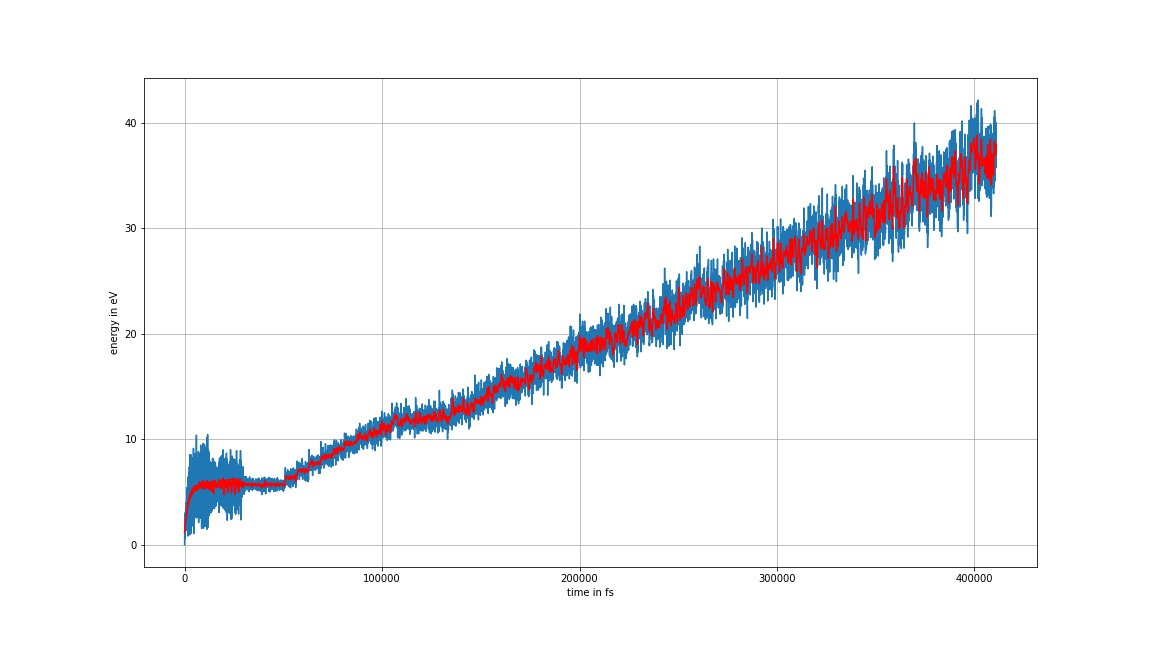
\includegraphics[scale=1]{/home/cm/CLionProjects/MoleDymCode/AData/Clusters/kineticEnergyCurve3.png} 
    \end{center} 
    \caption[Gold Cluster Simulation with 147 Atoms]{Gold Cluster Simulation with 147 Atoms} 
    \label{GoldClusterSimulationKineticTime147} 
\end{figure} 
 
\begin{figure}[!h] 
    \begin{center} 
        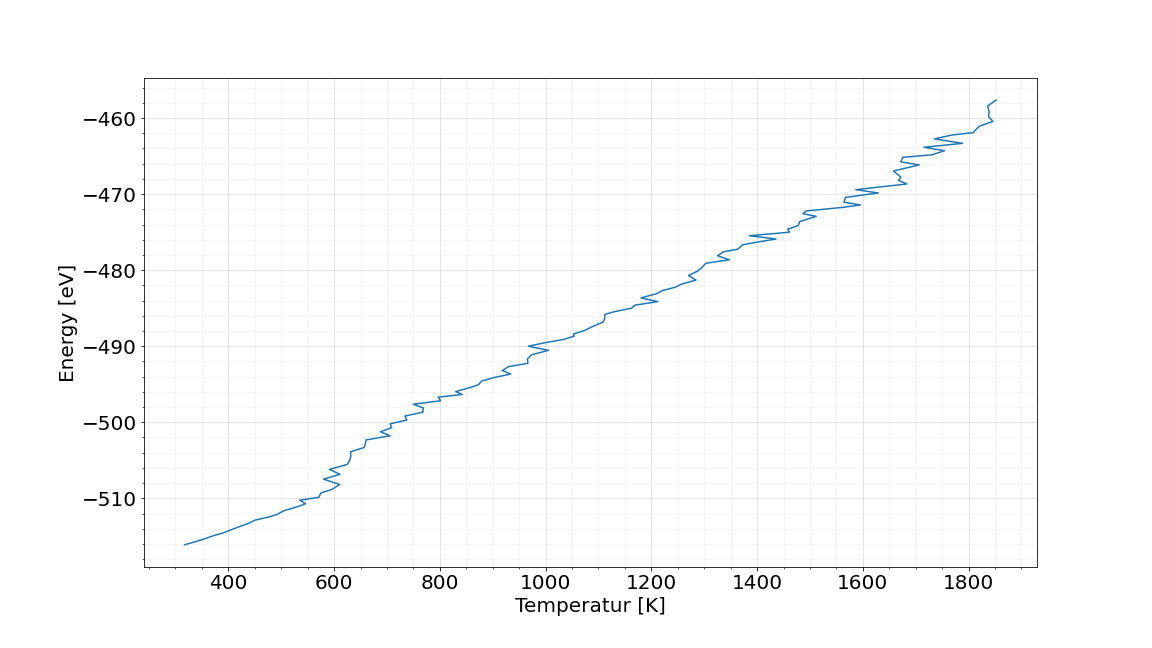
\includegraphics[scale=1]{/home/cm/CLionProjects/MoleDymCode/AData/Clusters/temperaturPotentialEnergyCurve3.png} 
    \end{center} 
    \caption[Gold Cluster Simulation with 147 Atoms]{Gold Cluster Simulation with 147 Atoms} 
    \label{GoldClusterSimulationTemperaturEnergy147} 
\end{figure} 
 
\begin{figure}[!h] 
    \begin{center} 
        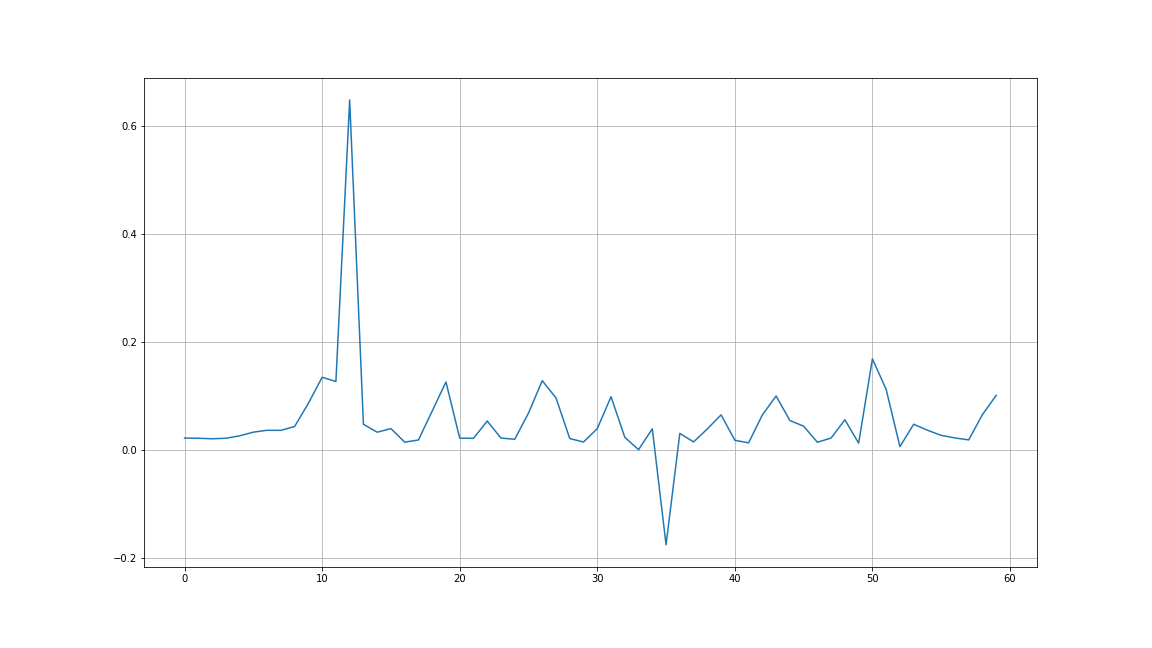
\includegraphics[scale=1]{/home/cm/CLionProjects/MoleDymCode/AData/Clusters/temperaturEnergyCurveGradients3.png} 
    \end{center} 
    \caption[Gradient of Temperatur and Energy for the Gold Cluster Simulation with 147 Atoms]{Gradient of Temperatur and Energy for the Gold Cluster Simulation with 147 Atoms} 
    \label{GoldClusterSimulationGradient147} 
\end{figure} 
 
% Figures for 309 Atoms 
\begin{figure}[!h] 
    \begin{center} 
        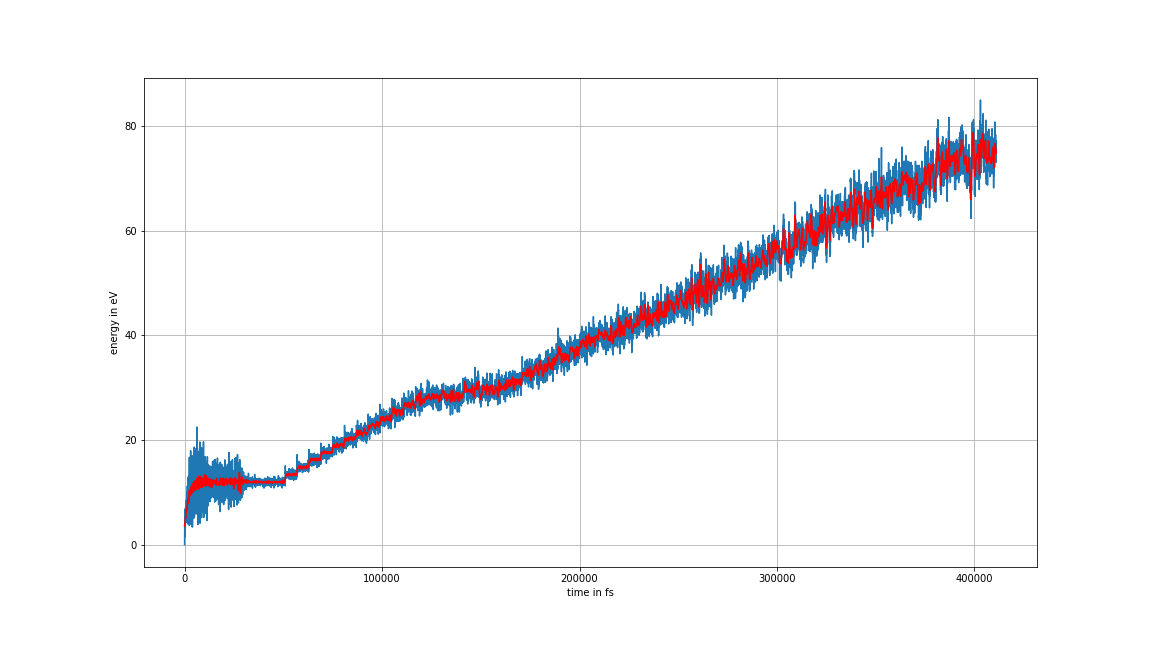
\includegraphics[scale=1]{/home/cm/CLionProjects/MoleDymCode/AData/Clusters/kineticEnergyCurve4.png} 
    \end{center} 
    \caption[Gold Cluster Simulation with 309 Atoms]{Gold Cluster Simulation with 309 Atoms} 
    \label{GoldClusterSimulationKineticTime309} 
\end{figure} 
 
\begin{figure}[!h] 
    \begin{center} 
        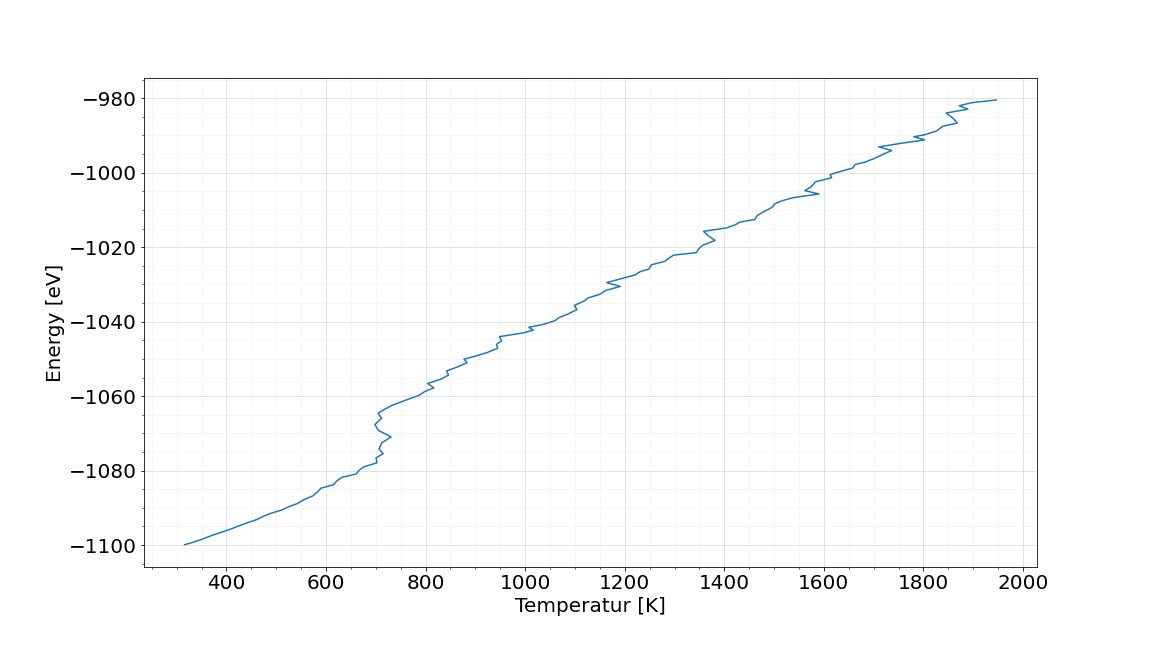
\includegraphics[scale=1]{/home/cm/CLionProjects/MoleDymCode/AData/Clusters/temperaturPotentialEnergyCurve4.png} 
    \end{center} 
    \caption[Gold Cluster Simulation with 309 Atoms]{Gold Cluster Simulation with 309 Atoms} 
    \label{GoldClusterSimulationTemperaturEnergy309} 
\end{figure} 
 
\begin{figure}[!h] 
    \begin{center} 
        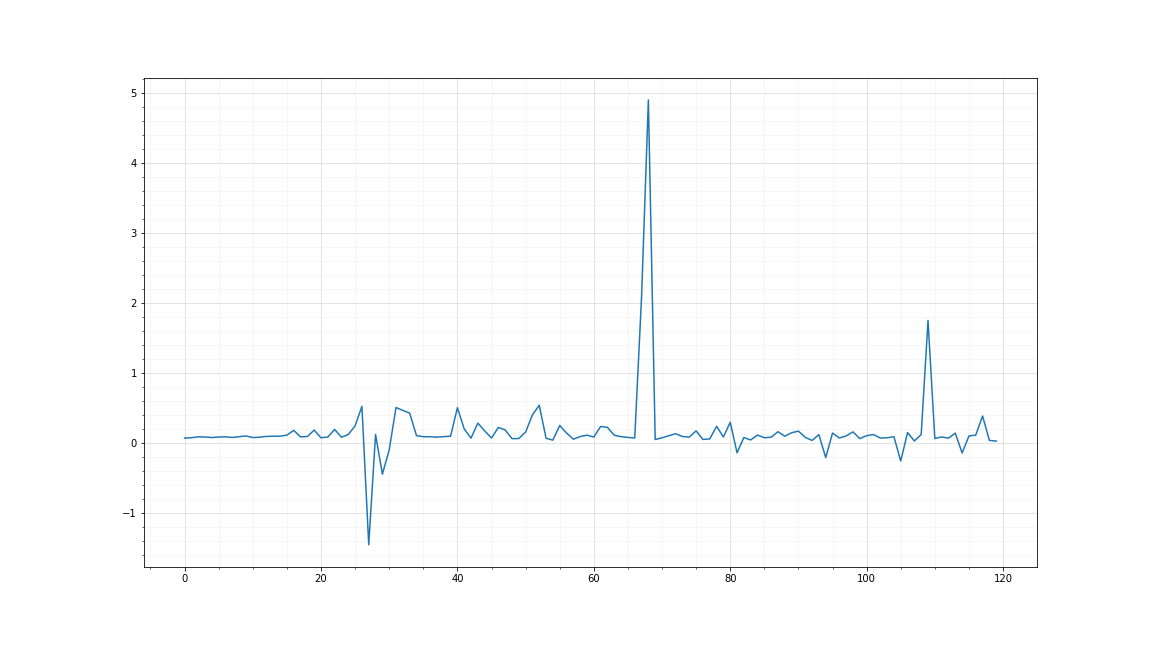
\includegraphics[scale=1]{/home/cm/CLionProjects/MoleDymCode/AData/Clusters/temperaturEnergyCurveGradients4.png} 
    \end{center} 
    \caption[Gradient of Temperatur and Energy for the Gold Cluster Simulation with 309 Atoms]{Gradient of Temperatur and Energy for the Gold Cluster Simulation with 309 Atoms} 
    \label{GoldClusterSimulationGradient309} 
\end{figure} 
 
% Figures for 561 Atoms 
\begin{figure}[!h] 
    \begin{center} 
        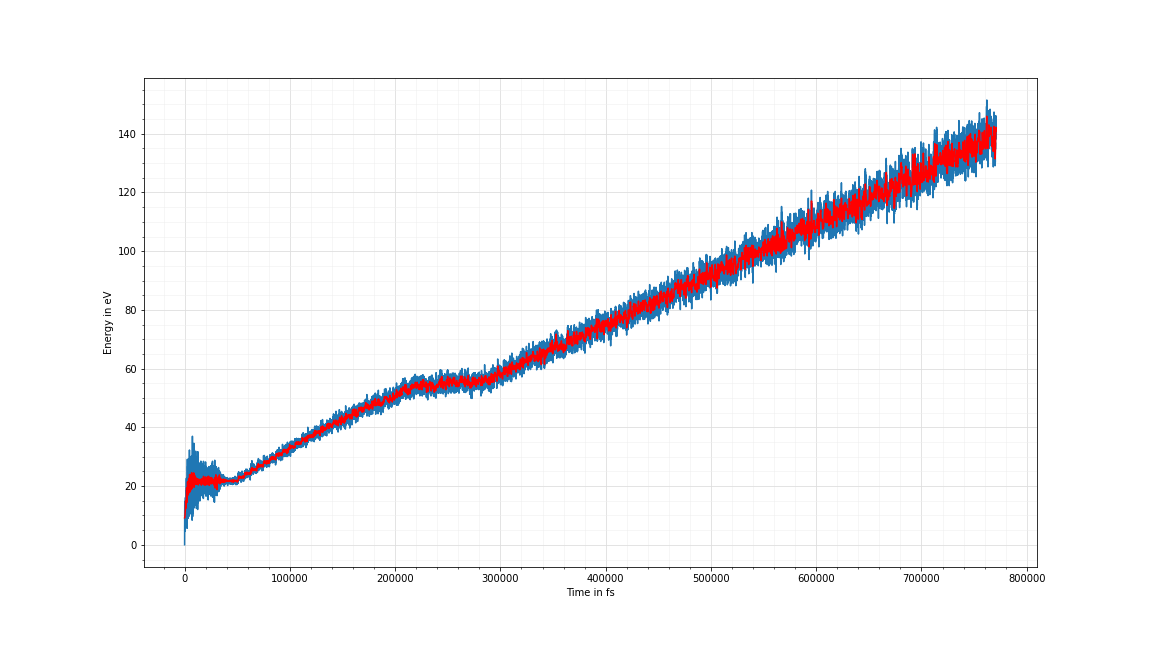
\includegraphics[scale=1]{/home/cm/CLionProjects/MoleDymCode/AData/Clusters/kineticEnergyCurve5.png} 
    \end{center} 
    \caption[Gold Cluster Simulation with 561 Atoms]{Gold Cluster Simulation with 561 Atoms} 
    \label{GoldClusterSimulationKineticTime561} 
\end{figure} 
 
\begin{figure}[!h] 
    \begin{center} 
        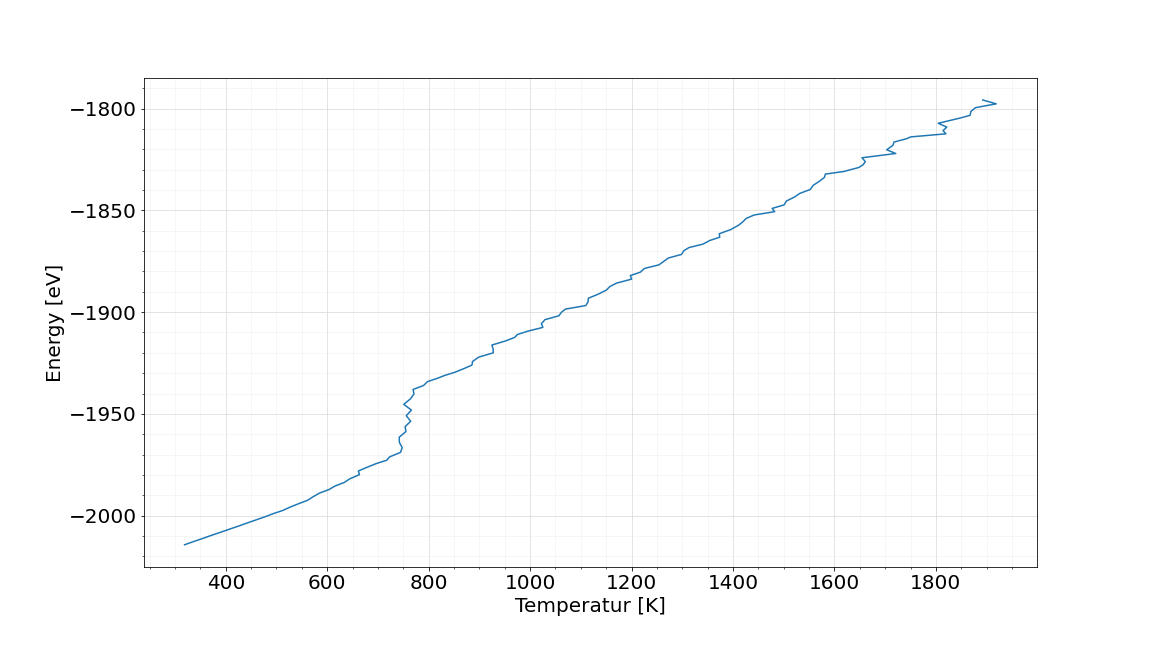
\includegraphics[scale=1]{/home/cm/CLionProjects/MoleDymCode/AData/Clusters/temperaturPotentialEnergyCurve5.png} 
    \end{center} 
    \caption[Gold Cluster Simulation with 561 Atoms]{Gold Cluster Simulation with 561 Atoms} 
    \label{GoldClusterSimulationTemperaturEnergy561} 
\end{figure} 
 
\begin{figure}[!h] 
    \begin{center} 
        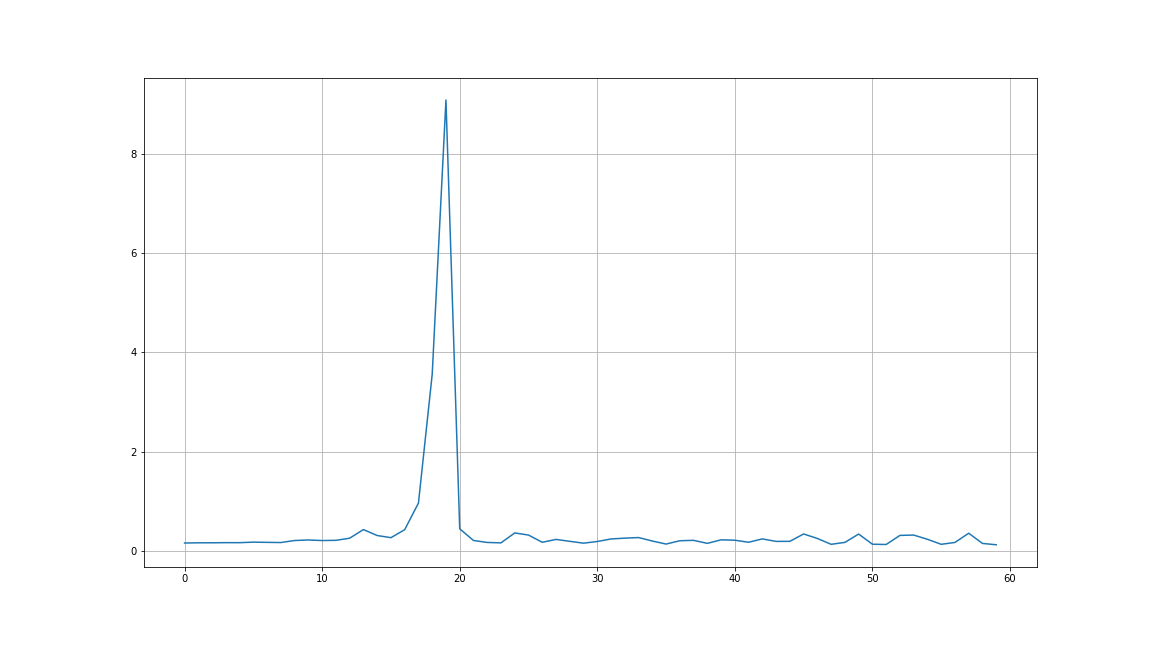
\includegraphics[scale=1]{/home/cm/CLionProjects/MoleDymCode/AData/Clusters/temperaturEnergyCurveGradients5.png} 
    \end{center} 
    \caption[Gradient of Temperatur and Energy for the Gold Cluster Simulation with 561 Atoms]{Gradient of Temperatur and Energy for the Gold Cluster Simulation with 561 Atoms} 
    \label{GoldClusterSimulationGradient561} 
\end{figure} 
 
% Figures for 923 Atoms 
\begin{figure}[!h] 
    \begin{center} 
        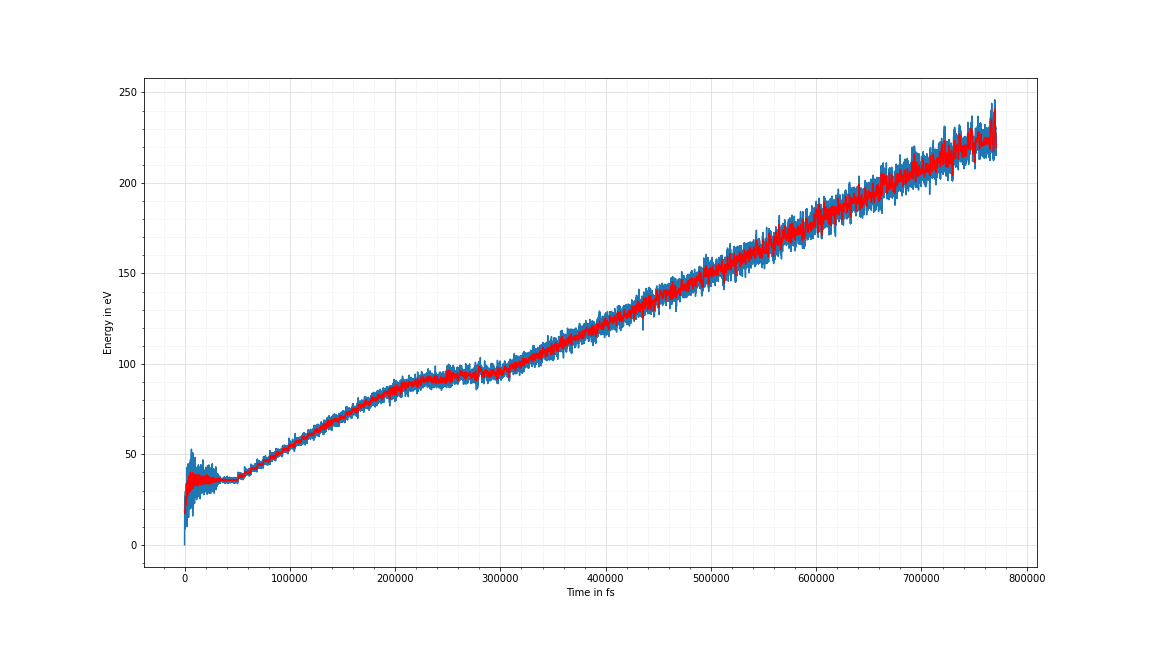
\includegraphics[scale=1]{/home/cm/CLionProjects/MoleDymCode/AData/Clusters/kineticEnergyCurve6.png} 
    \end{center} 
    \caption[Gold Cluster Simulation with 923 Atoms]{Gold Cluster Simulation with 923 Atoms} 
    \label{GoldClusterSimulationKineticTime923} 
\end{figure} 
 
\begin{figure}[!h] 
    \begin{center} 
        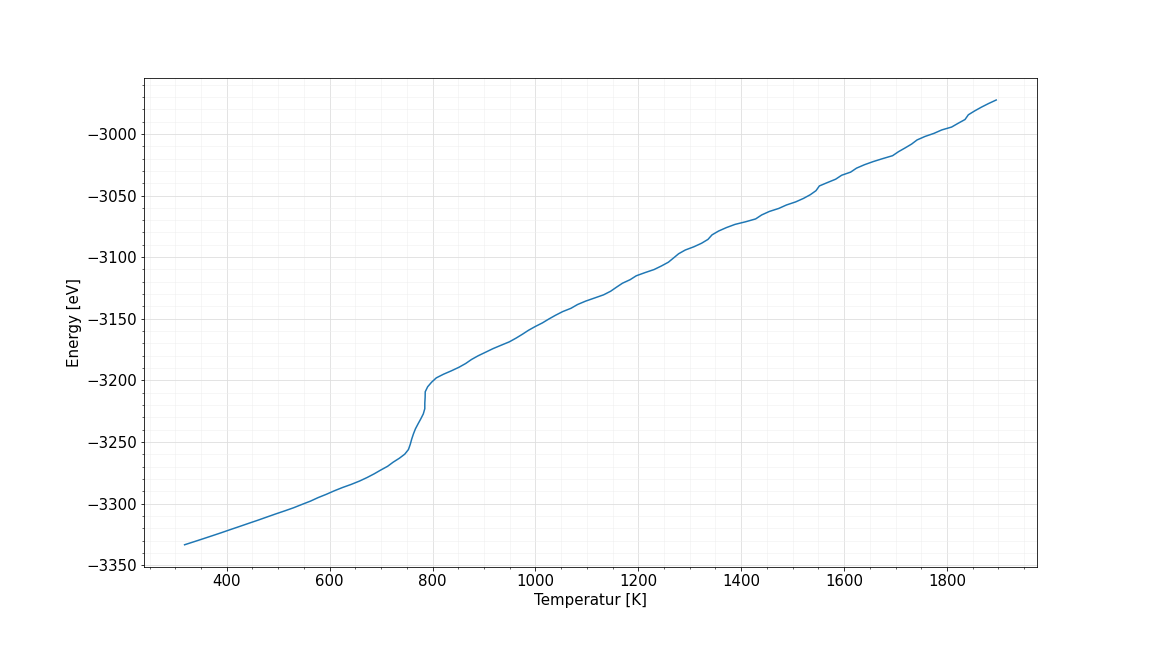
\includegraphics[scale=1]{/home/cm/CLionProjects/MoleDymCode/AData/Clusters/temperaturPotentialEnergyCurve6.png} 
    \end{center} 
    \caption[Gold Cluster Simulation with 923 Atoms]{Gold Cluster Simulation with 923 Atoms} 
    \label{GoldClusterSimulationTemperaturEnergy923} 
\end{figure} 
 
\begin{figure}[!h] 
    \begin{center} 
        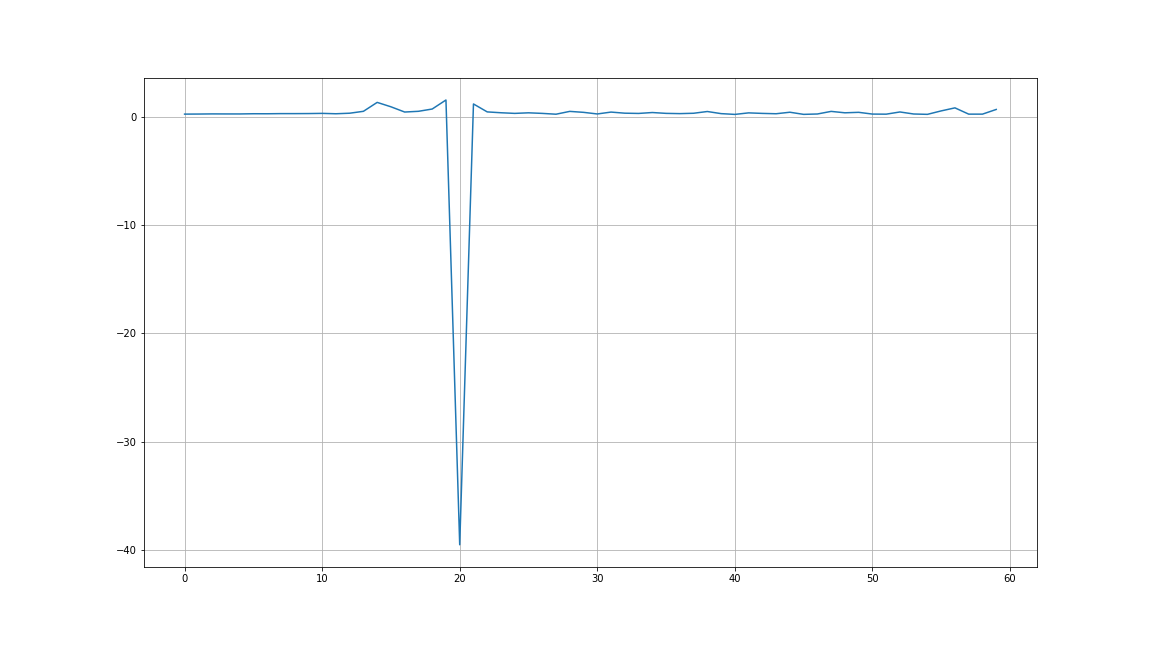
\includegraphics[scale=1]{/home/cm/CLionProjects/MoleDymCode/AData/Clusters/temperaturEnergyCurveGradients6.png} 
    \end{center} 
    \caption[Gradient of Temperatur and Energy for the Gold Cluster Simulation with 923 Atoms]{Gradient of Temperatur and Energy for the Gold Cluster Simulation with 923 Atoms} 
    \label{GoldClusterSimulationGradient923} 
\end{figure} 
 
% Figures for 1415 Atoms 
\begin{figure}[!h] 
    \begin{center} 
        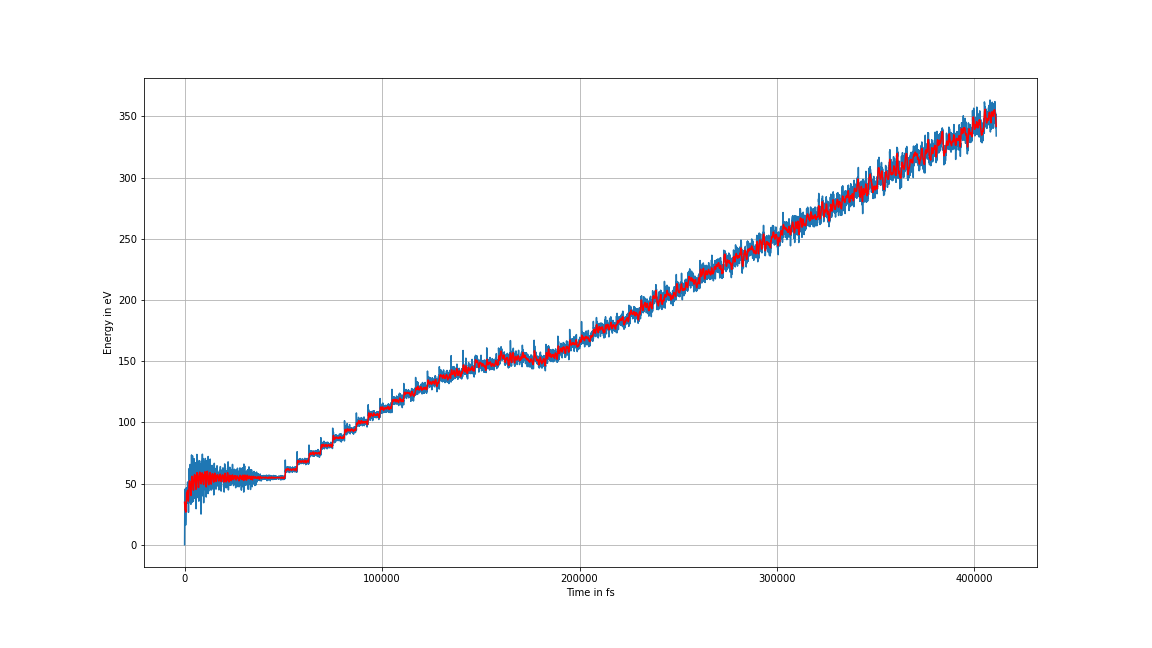
\includegraphics[scale=1]{/home/cm/CLionProjects/MoleDymCode/AData/Clusters/kineticEnergyCurve7.png} 
    \end{center} 
    \caption[Gold Cluster Simulation with 1415 Atoms]{Gold Cluster Simulation with 1415 Atoms} 
    \label{GoldClusterSimulationKineticTime1415} 
\end{figure} 
 
\begin{figure}[!h] 
    \begin{center} 
        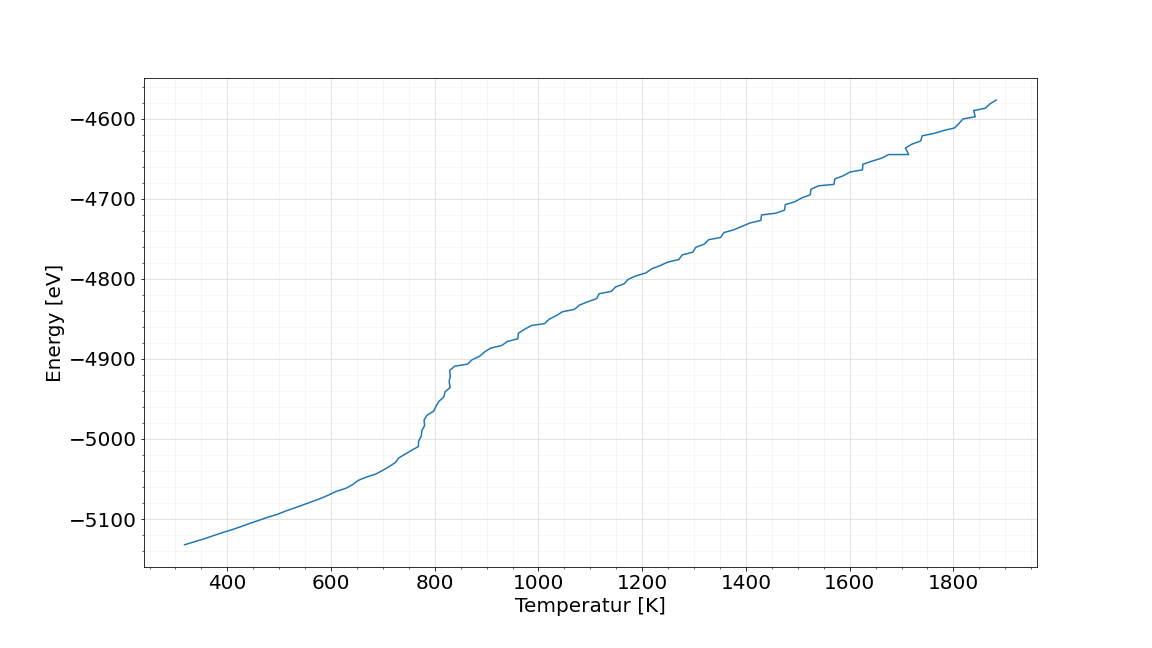
\includegraphics[scale=1]{/home/cm/CLionProjects/MoleDymCode/AData/Clusters/temperaturPotentialEnergyCurve7.png} 
    \end{center} 
    \caption[Gold Cluster Simulation with 1415 Atoms]{Gold Cluster Simulation with 1415 Atoms} 
    \label{GoldClusterSimulationTemperaturEnergy1415} 
\end{figure} 
 
\begin{figure}[!h] 
    \begin{center} 
        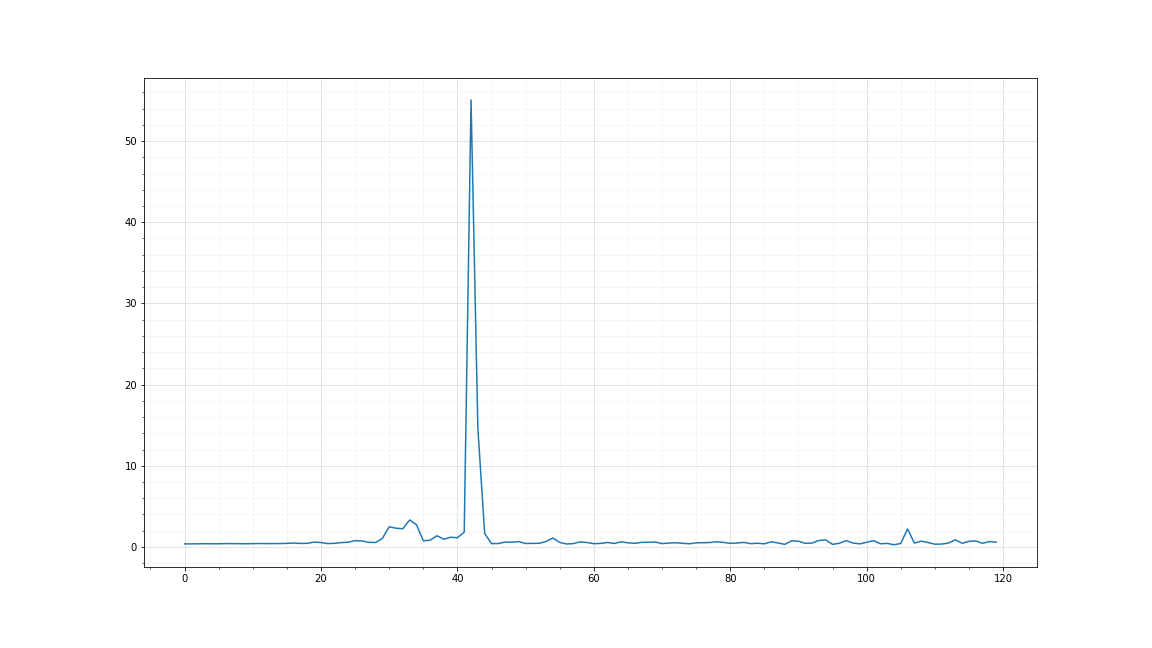
\includegraphics[scale=1]{/home/cm/CLionProjects/MoleDymCode/AData/Clusters/temperaturEnergyCurveGradients7.png} 
    \end{center} 
    \caption[Gradient of Temperatur and Energy for the Gold Cluster Simulation with 1415 Atoms]{Gradient of Temperatur and Energy for the Gold Cluster Simulation with 1415 Atoms} 
    \label{GoldClusterSimulationGradient1415} 
\end{figure} 
 
% Figures for 2057 Atoms 
\begin{figure}[!h] 
    \begin{center} 
        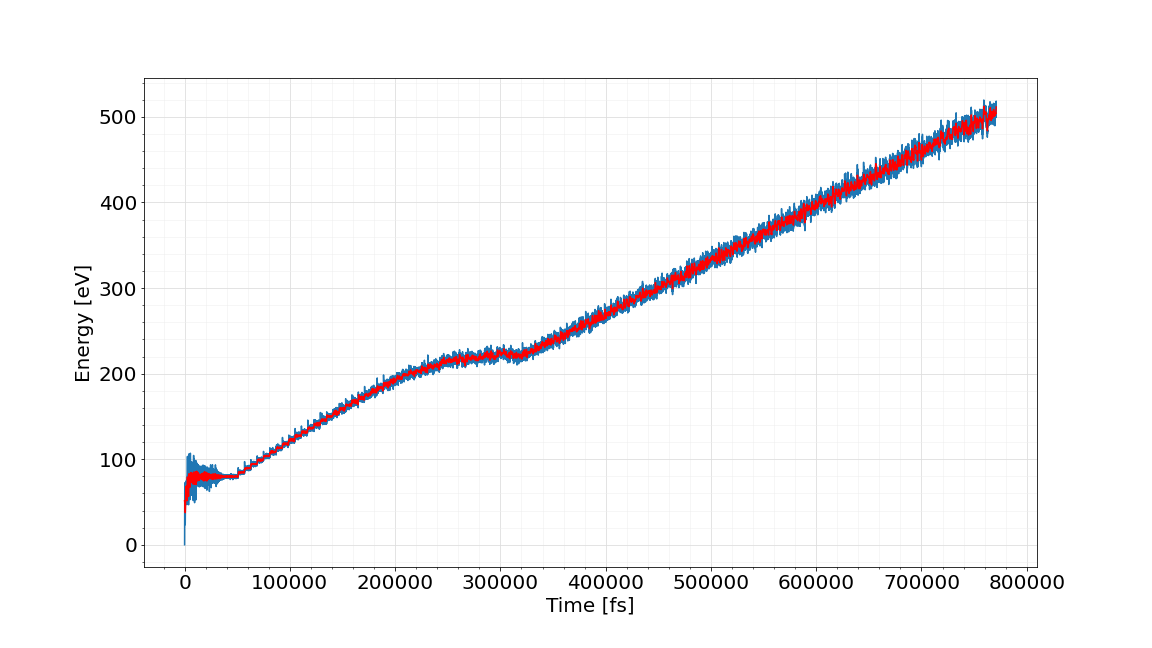
\includegraphics[scale=1]{/home/cm/CLionProjects/MoleDymCode/AData/Clusters/kineticEnergyCurve8.png} 
    \end{center} 
    \caption[Gold Cluster Simulation with 2057 Atoms]{Gold Cluster Simulation with 2057 Atoms} 
    \label{GoldClusterSimulationKineticTime2057} 
\end{figure} 
 
\begin{figure}[!h] 
    \begin{center} 
        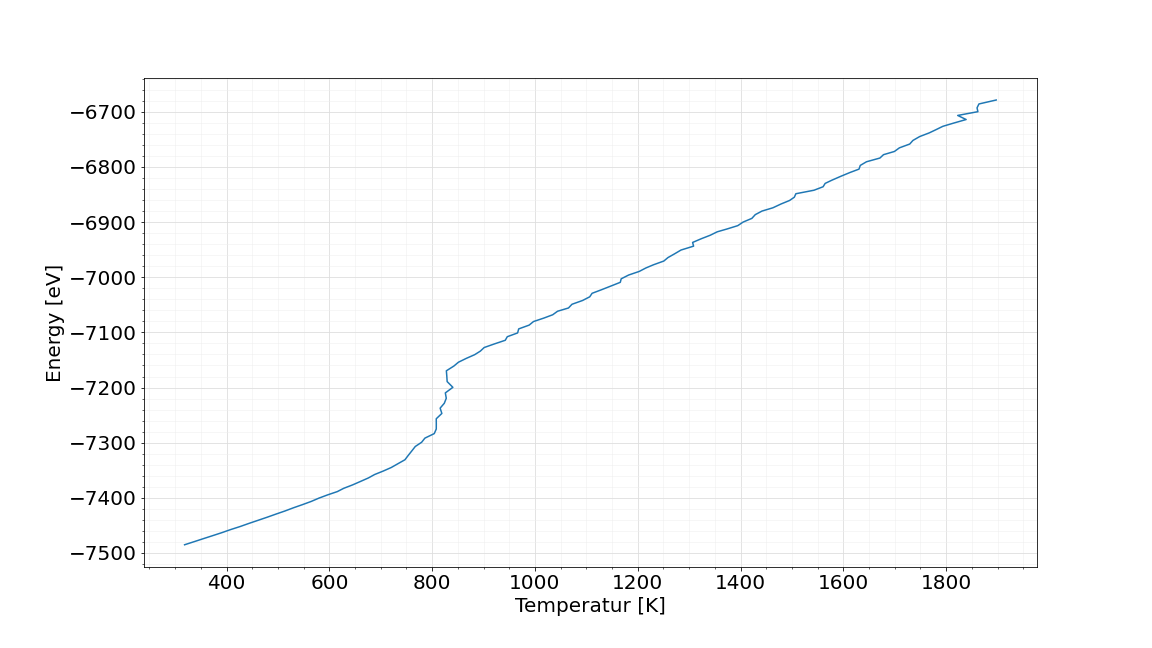
\includegraphics[scale=1]{/home/cm/CLionProjects/MoleDymCode/AData/Clusters/temperaturPotentialEnergyCurve8.png} 
    \end{center} 
    \caption[Gold Cluster Simulation with 2057 Atoms]{Gold Cluster Simulation with 2057 Atoms} 
    \label{GoldClusterSimulationTemperaturEnergy2057} 
\end{figure} 
 
\begin{figure}[!h] 
    \begin{center} 
        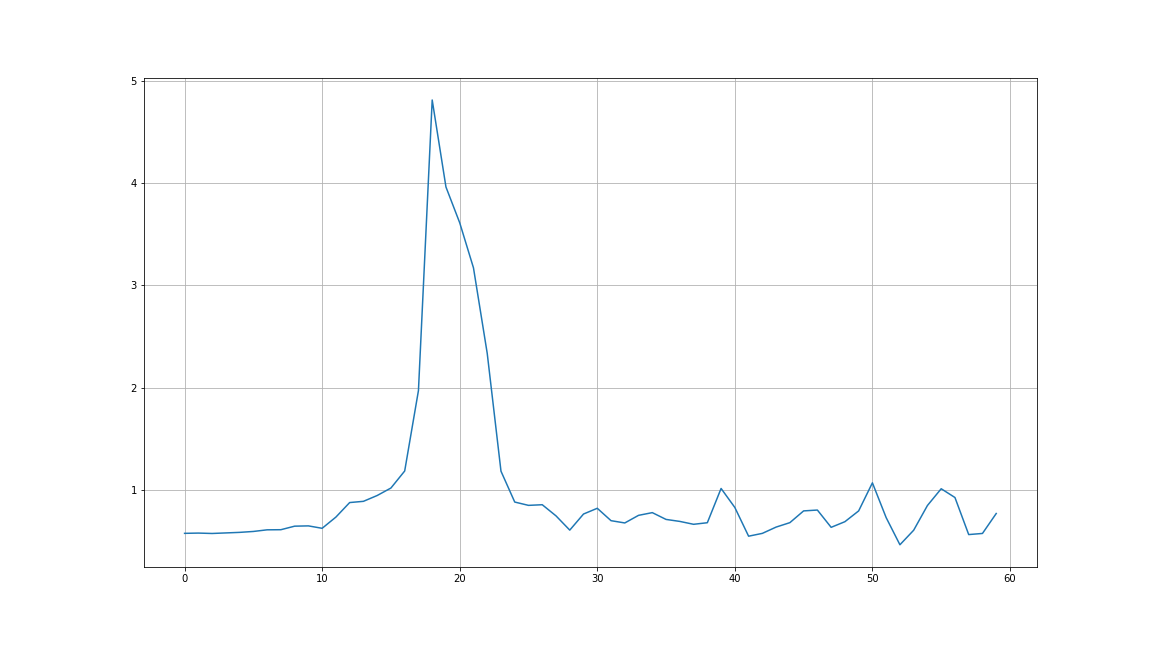
\includegraphics[scale=1]{/home/cm/CLionProjects/MoleDymCode/AData/Clusters/temperaturEnergyCurveGradients8.png} 
    \end{center} 
    \caption[Gradient of Temperatur and Energy for the Gold Cluster Simulation with 2057 Atoms]{Gradient of Temperatur and Energy for the Gold Cluster Simulation with 2057 Atoms} 
    \label{GoldClusterSimulationGradient2057} 
\end{figure} 
 
% Figures for 2869 Atoms 
\begin{figure}[!h] 
    \begin{center} 
        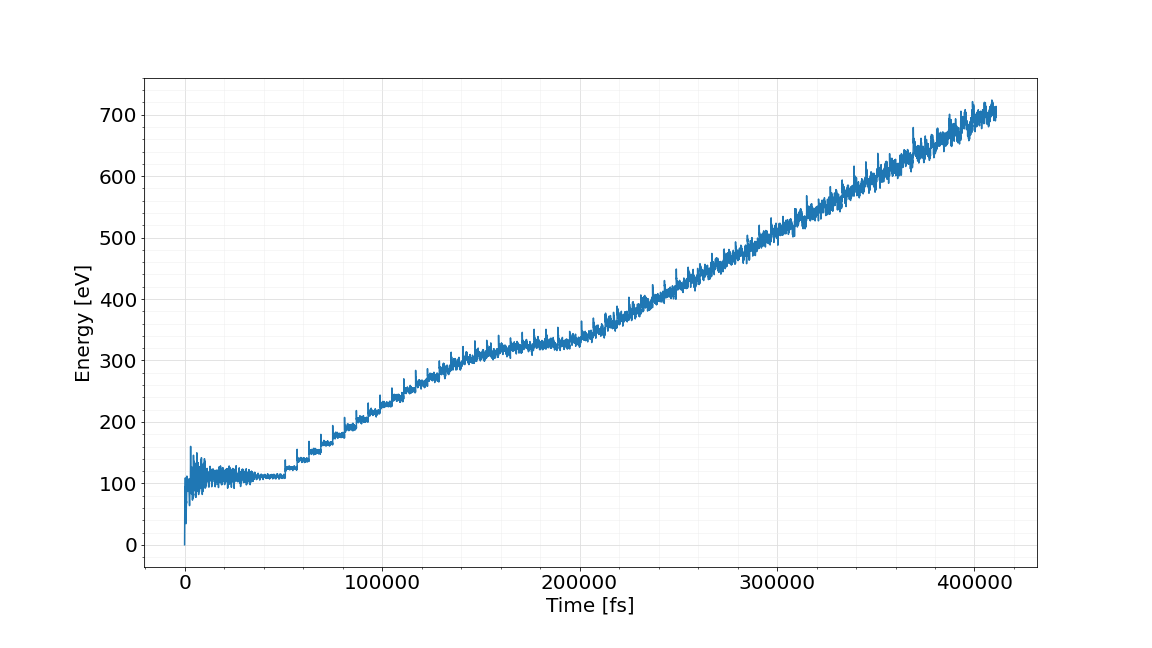
\includegraphics[scale=1]{/home/cm/CLionProjects/MoleDymCode/AData/Clusters/kineticEnergyCurve9.png} 
    \end{center} 
    \caption[Gold Cluster Simulation with 2869 Atoms]{Gold Cluster Simulation with 2869 Atoms} 
    \label{GoldClusterSimulationKineticTime2869} 
\end{figure} 
 
\begin{figure}[!h] 
    \begin{center} 
        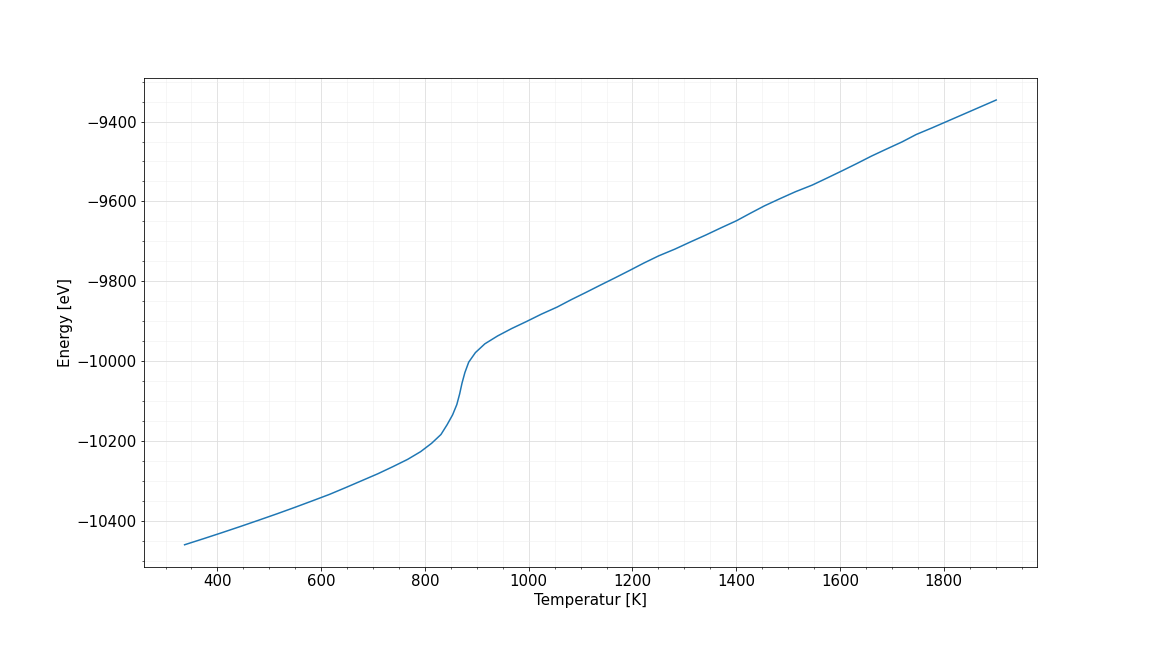
\includegraphics[scale=1]{/home/cm/CLionProjects/MoleDymCode/AData/Clusters/temperaturPotentialEnergyCurve9.png} 
    \end{center} 
    \caption[Gold Cluster Simulation with 2869 Atoms]{Gold Cluster Simulation with 2869 Atoms} 
    \label{GoldClusterSimulationTemperaturEnergy2869} 
\end{figure} 
 
\begin{figure}[!h] 
    \begin{center} 
        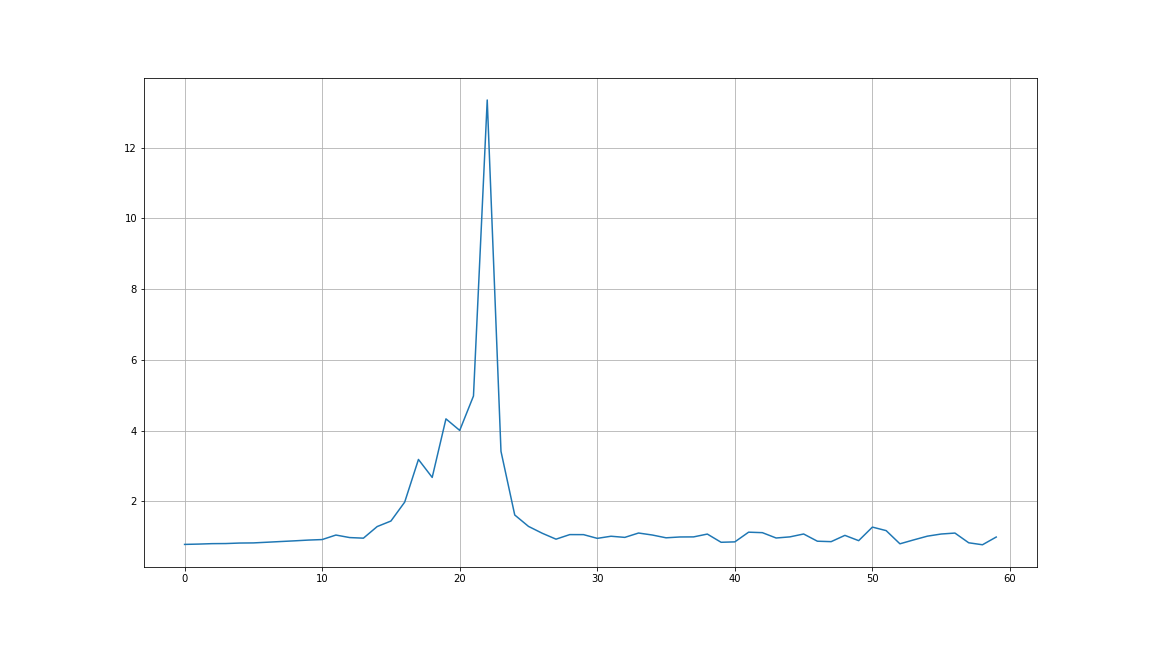
\includegraphics[scale=1]{/home/cm/CLionProjects/MoleDymCode/AData/Clusters/temperaturEnergyCurveGradients9.png} 
    \end{center} 
    \caption[Gradient of Temperatur and Energy for the Gold Cluster Simulation with 2869 Atoms]{Gradient of Temperatur and Energy for the Gold Cluster Simulation with 2869 Atoms} 
    \label{GoldClusterSimulationGradient2869} 
\end{figure} 
 
% Figures for 3871 Atoms 
\begin{figure}[!h] 
    \begin{center} 
        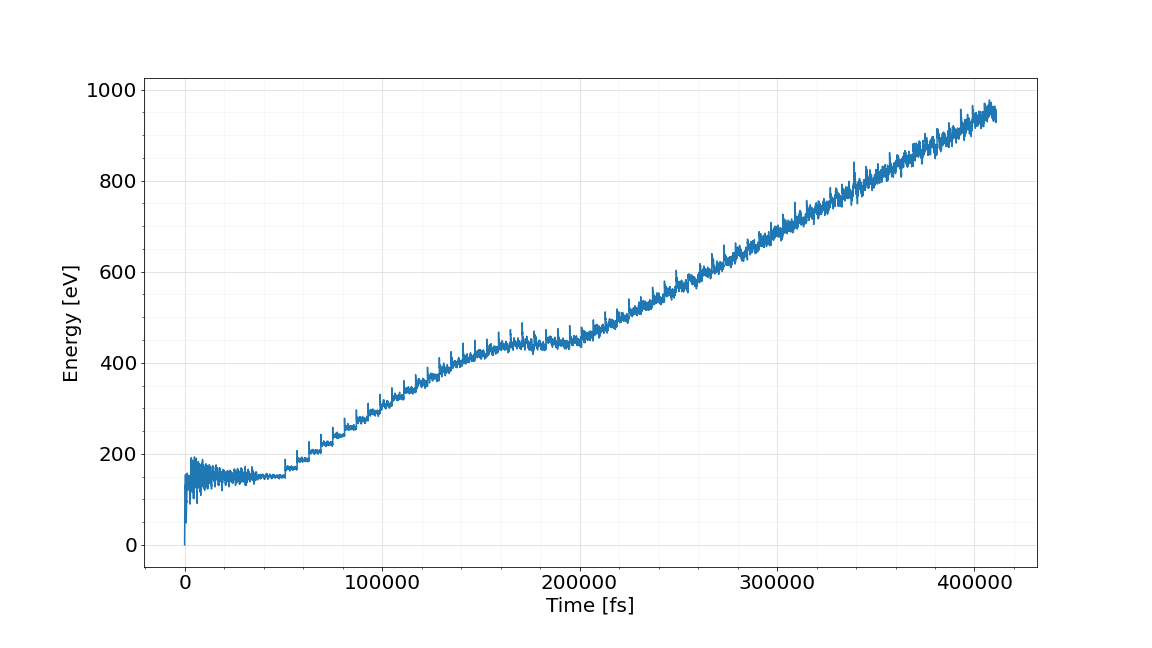
\includegraphics[scale=1]{/home/cm/CLionProjects/MoleDymCode/AData/Clusters/kineticEnergyCurve10.png} 
    \end{center} 
    \caption[Gold Cluster Simulation with 3871 Atoms]{Gold Cluster Simulation with 3871 Atoms} 
    \label{GoldClusterSimulationKineticTime3871} 
\end{figure} 
 
\begin{figure}[!h] 
    \begin{center} 
        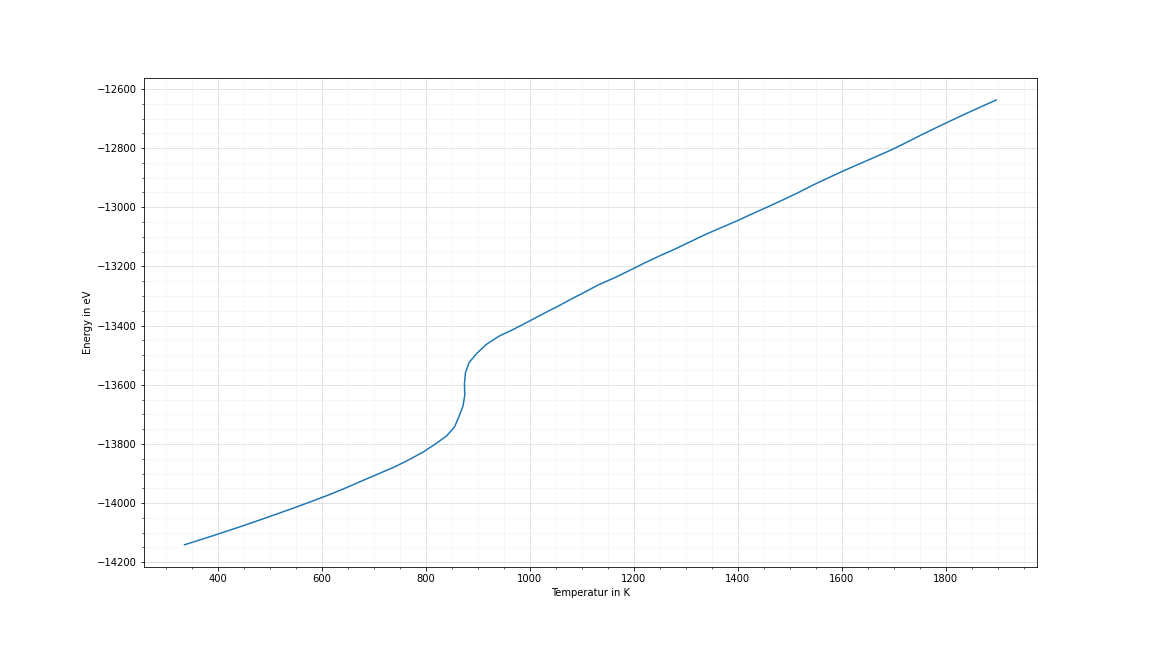
\includegraphics[scale=1]{/home/cm/CLionProjects/MoleDymCode/AData/Clusters/temperaturPotentialEnergyCurve10.png} 
    \end{center} 
    \caption[Gold Cluster Simulation with 3871 Atoms]{Gold Cluster Simulation with 3871 Atoms} 
    \label{GoldClusterSimulationTemperaturEnergy3871} 
\end{figure} 
 
\begin{figure}[!h] 
    \begin{center} 
        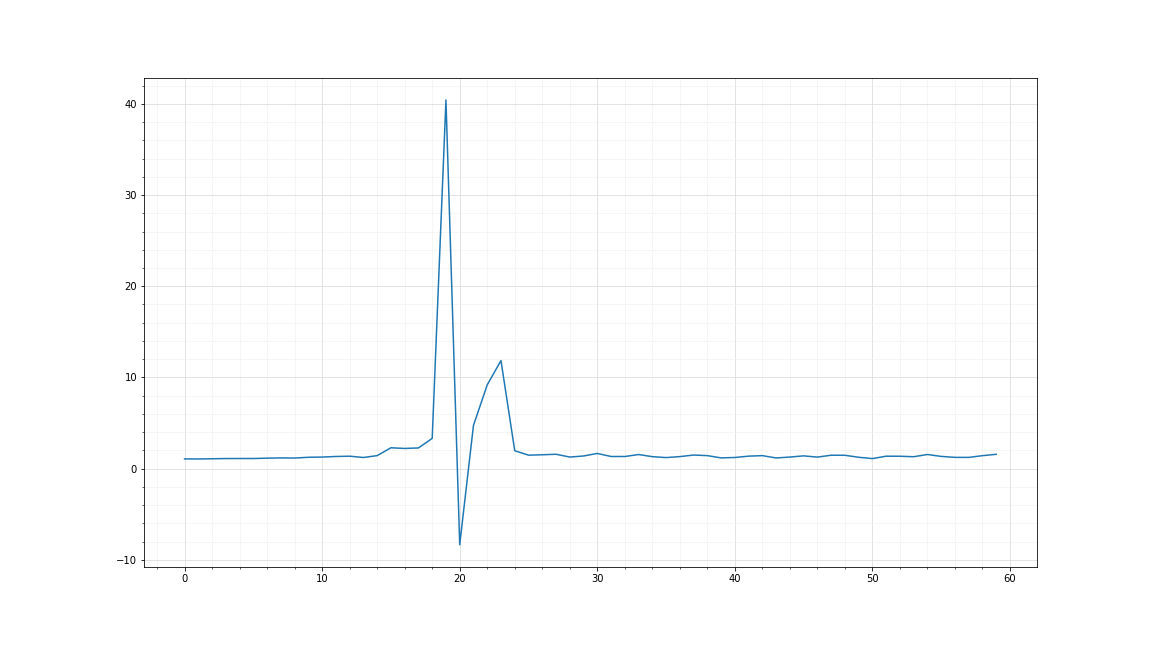
\includegraphics[scale=1]{/home/cm/CLionProjects/MoleDymCode/AData/Clusters/temperaturEnergyCurveGradients10.png} 
    \end{center} 
    \caption[Gradient of Temperatur and Energy for the Gold Cluster Simulation with 3871 Atoms]{Gradient of Temperatur and Energy for the Gold Cluster Simulation with 3871 Atoms} 
    \label{GoldClusterSimulationGradient3871} 
\end{figure} 
 
% Figures for 5083 Atoms 
\begin{figure}[!h] 
    \begin{center} 
        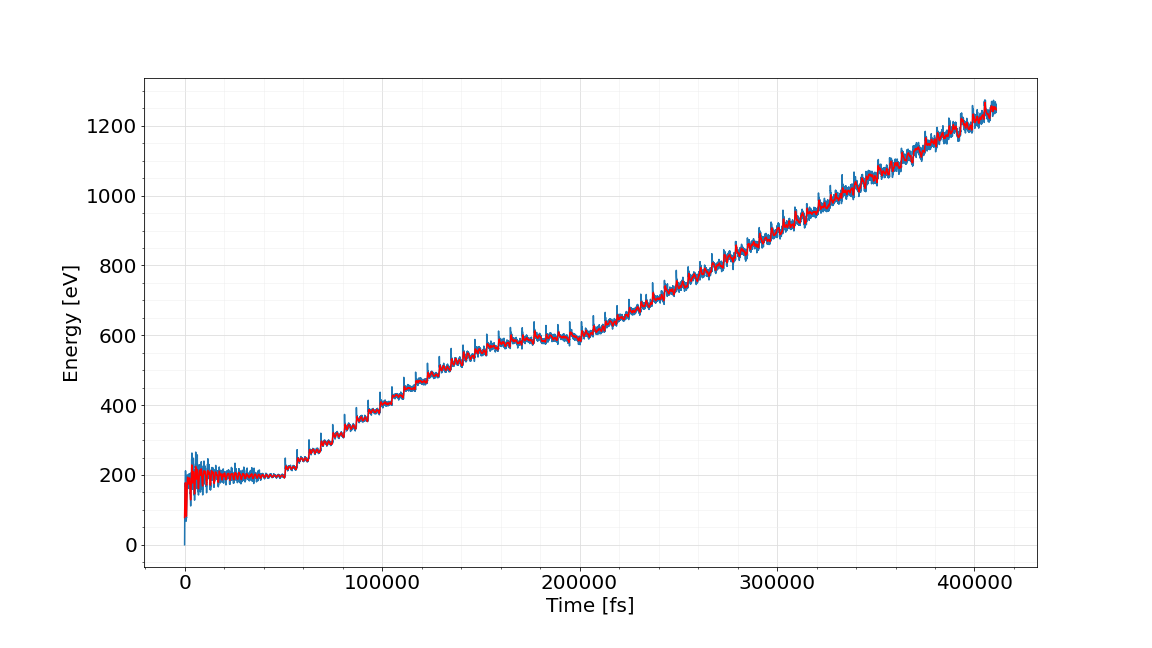
\includegraphics[scale=1]{/home/cm/CLionProjects/MoleDymCode/AData/Clusters/kineticEnergyCurve11.png} 
    \end{center} 
    \caption[Gold Cluster Simulation with 5083 Atoms]{Gold Cluster Simulation with 5083 Atoms} 
    \label{GoldClusterSimulationKineticTime5083} 
\end{figure} 
 
\begin{figure}[!h] 
    \begin{center} 
        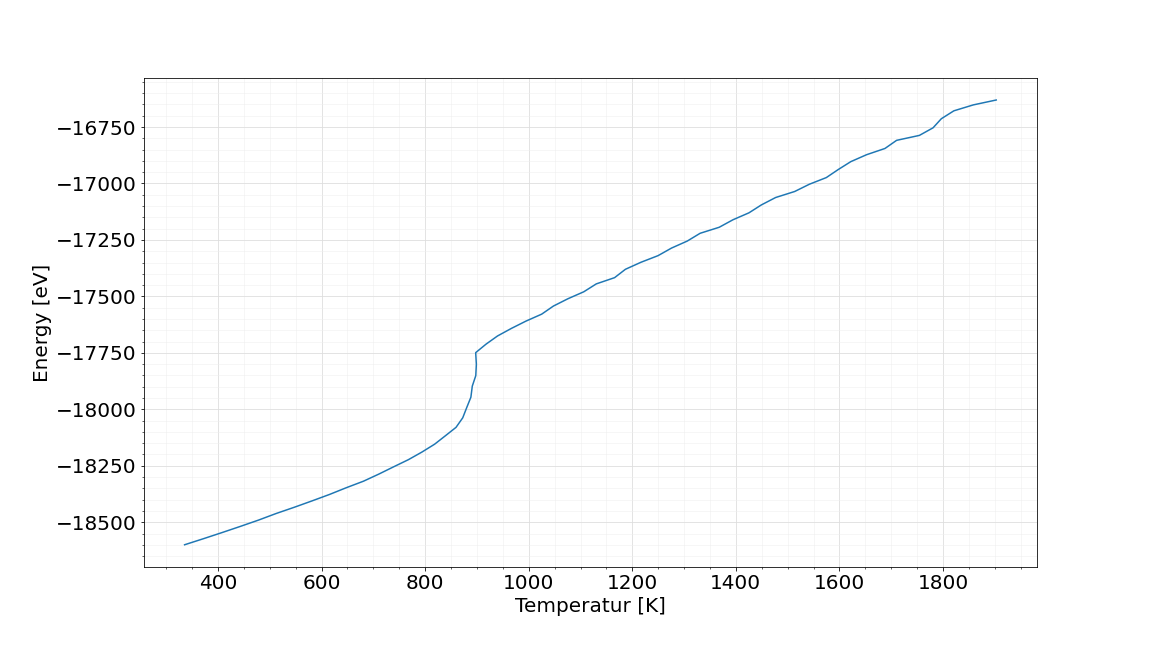
\includegraphics[scale=1]{/home/cm/CLionProjects/MoleDymCode/AData/Clusters/temperaturPotentialEnergyCurve11.png} 
    \end{center} 
    \caption[Gold Cluster Simulation with 5083 Atoms]{Gold Cluster Simulation with 5083 Atoms} 
    \label{GoldClusterSimulationTemperaturEnergy5083} 
\end{figure} 
 
\begin{figure}[!h] 
    \begin{center} 
        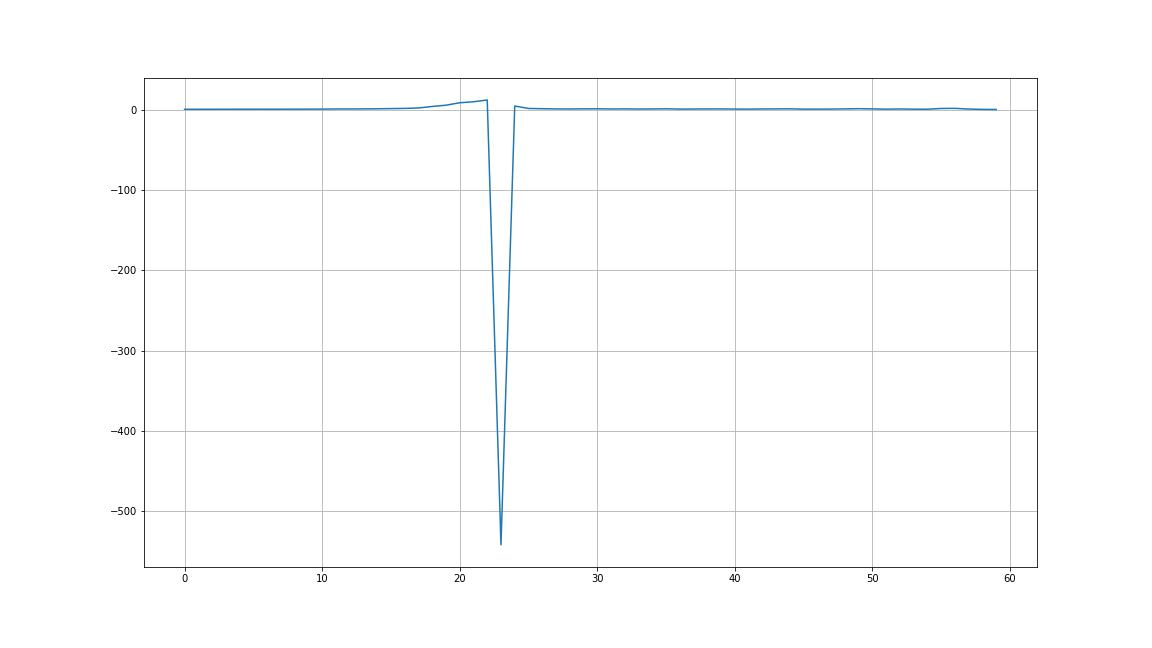
\includegraphics[scale=1]{/home/cm/CLionProjects/MoleDymCode/AData/Clusters/temperaturEnergyCurveGradients11.png} 
    \end{center} 
    \caption[Gradient of Temperatur and Energy for the Gold Cluster Simulation with 5083 Atoms]{Gradient of Temperatur and Energy for the Gold Cluster Simulation with 5083 Atoms} 
    \label{GoldClusterSimulationGradient5083} 
\end{figure} 
 
% Figures for 6525 Atoms 
\begin{figure}[!h] 
    \begin{center} 
        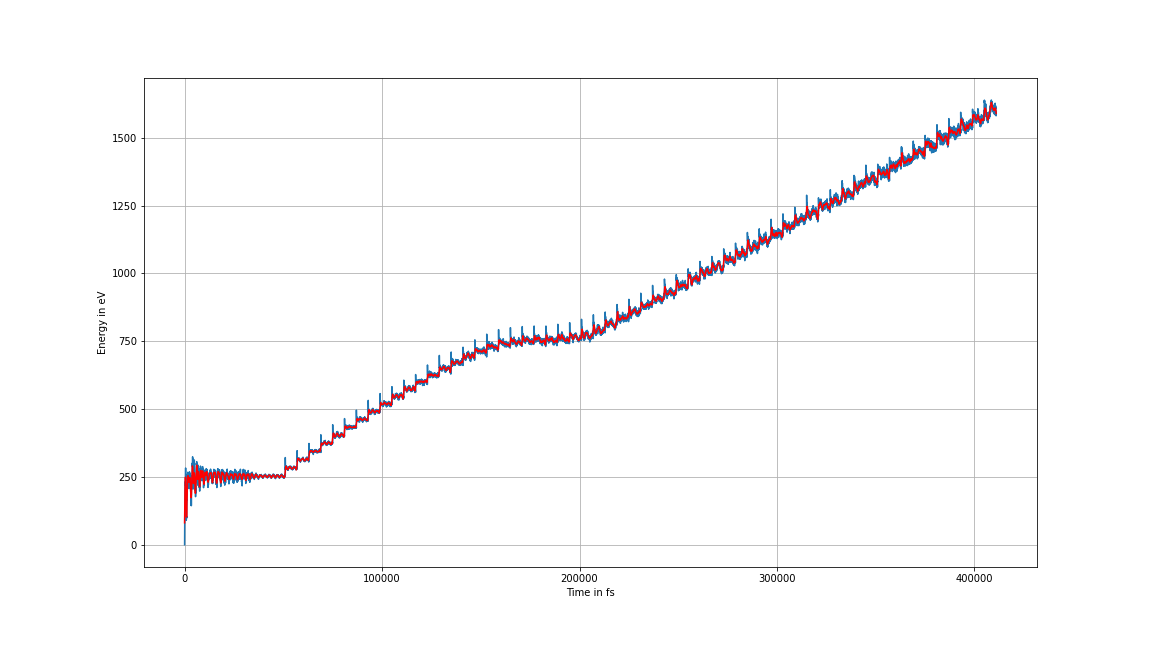
\includegraphics[scale=1]{/home/cm/CLionProjects/MoleDymCode/AData/Clusters/kineticEnergyCurve12.png} 
    \end{center} 
    \caption[Gold Cluster Simulation with 6525 Atoms]{Gold Cluster Simulation with 6525 Atoms} 
    \label{GoldClusterSimulationKineticTime6525} 
\end{figure} 
 
\begin{figure}[!h] 
    \begin{center} 
        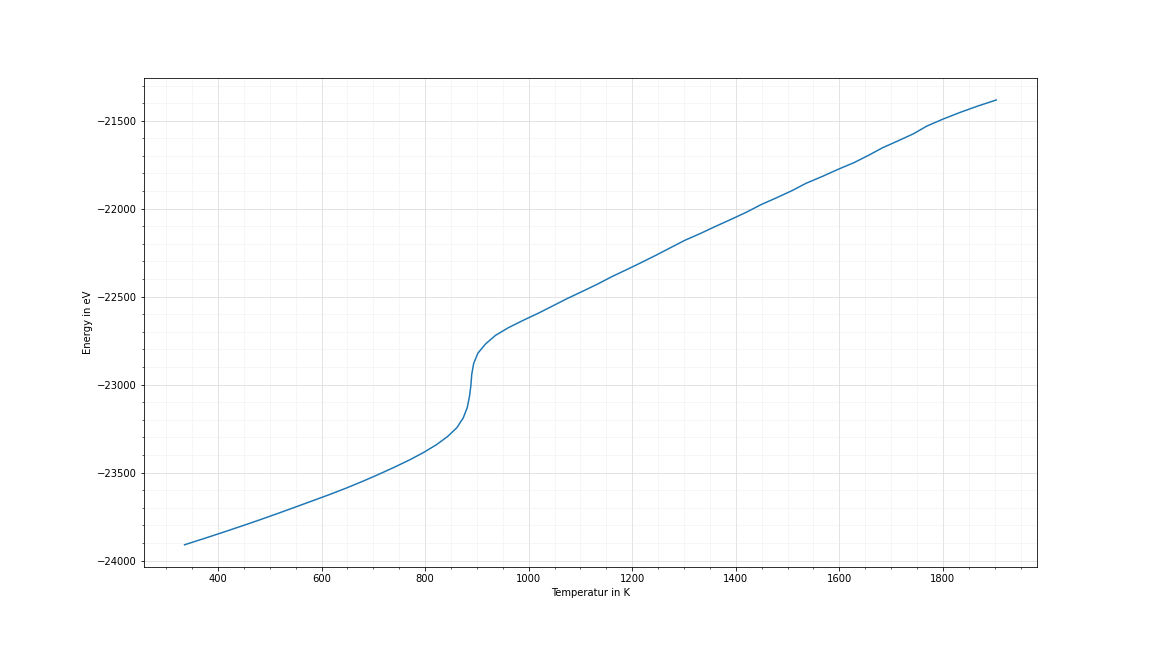
\includegraphics[scale=1]{/home/cm/CLionProjects/MoleDymCode/AData/Clusters/temperaturPotentialEnergyCurve12.png} 
    \end{center} 
    \caption[Gold Cluster Simulation with 6525 Atoms]{Gold Cluster Simulation with 6525 Atoms} 
    \label{GoldClusterSimulationTemperaturEnergy6525} 
\end{figure} 
 
\begin{figure}[!h] 
    \begin{center} 
        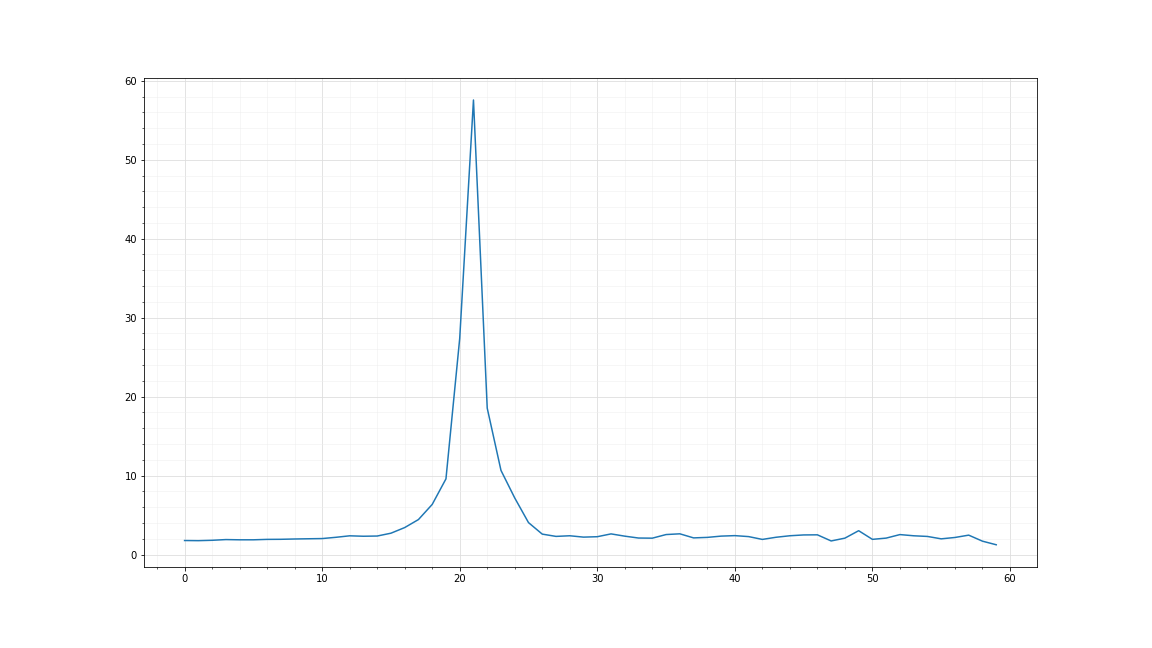
\includegraphics[scale=1]{/home/cm/CLionProjects/MoleDymCode/AData/Clusters/temperaturEnergyCurveGradients12.png} 
    \end{center} 
    \caption[Gradient of Temperatur and Energy for the Gold Cluster Simulation with 6525 Atoms]{Gradient of Temperatur and Energy for the Gold Cluster Simulation with 6525 Atoms} 
    \label{GoldClusterSimulationGradient6525} 
\end{figure} 
 
% Figures for 8217 Atoms 
\begin{figure}[!h] 
    \begin{center} 
        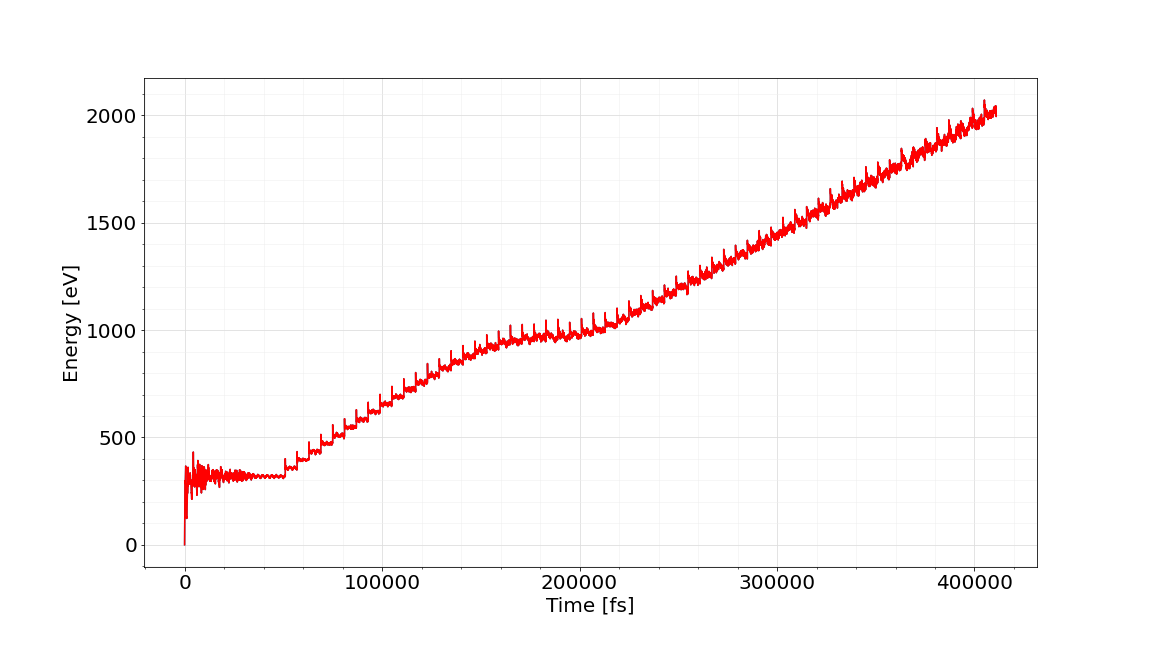
\includegraphics[scale=1]{/home/cm/CLionProjects/MoleDymCode/AData/Clusters/kineticEnergyCurve13.png} 
    \end{center} 
    \caption[Gold Cluster Simulation with 8217 Atoms]{Gold Cluster Simulation with 8217 Atoms} 
    \label{GoldClusterSimulationKineticTime8217} 
\end{figure} 
 
\begin{figure}[!h] 
    \begin{center} 
        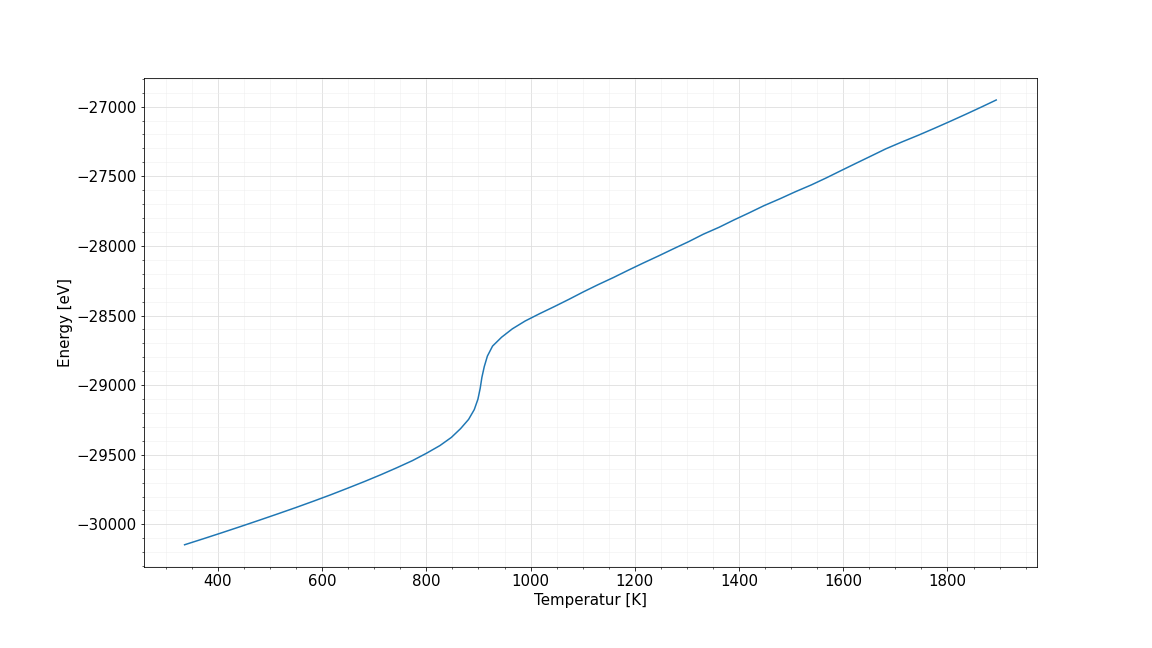
\includegraphics[scale=1]{/home/cm/CLionProjects/MoleDymCode/AData/Clusters/temperaturPotentialEnergyCurve13.png} 
    \end{center} 
    \caption[Gold Cluster Simulation with 8217 Atoms]{Gold Cluster Simulation with 8217 Atoms} 
    \label{GoldClusterSimulationTemperaturEnergy8217} 
\end{figure} 
 
\begin{figure}[!h] 
    \begin{center} 
        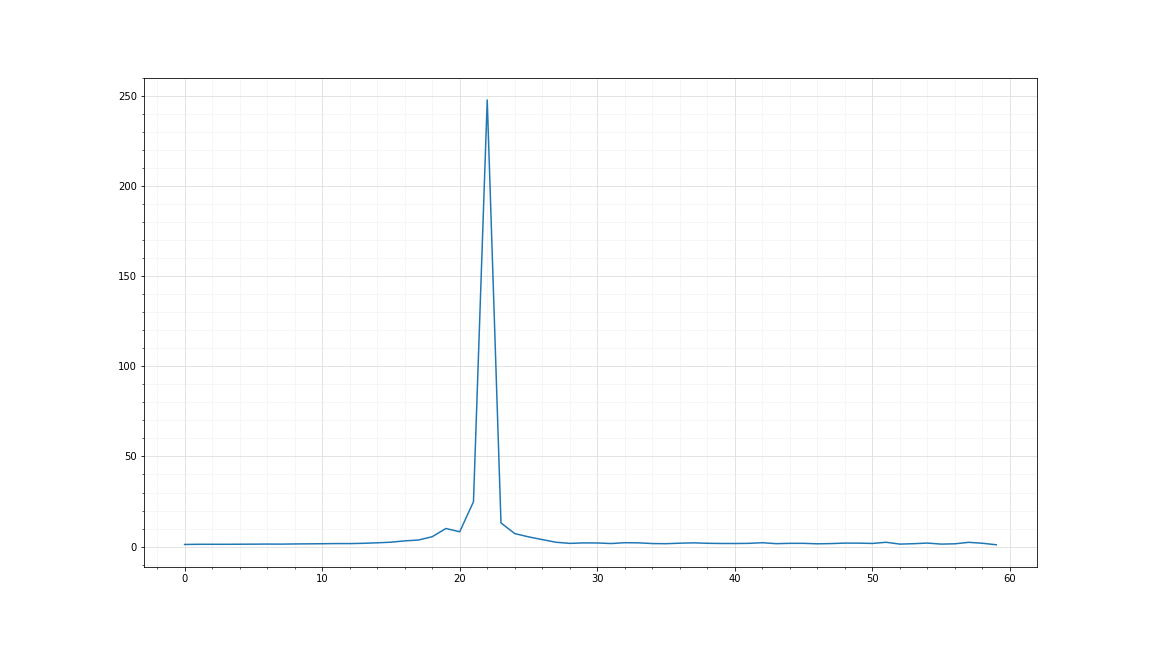
\includegraphics[scale=1]{/home/cm/CLionProjects/MoleDymCode/AData/Clusters/temperaturEnergyCurveGradients13.png} 
    \end{center} 
    \caption[Gradient of Temperatur and Energy for the Gold Cluster Simulation with 8217 Atoms]{Gradient of Temperatur and Energy for the Gold Cluster Simulation with 8217 Atoms} 
    \label{GoldClusterSimulationGradient8217} 
\end{figure} 
 
% Figures for 10179 Atoms 
\begin{figure}[!h] 
    \begin{center} 
        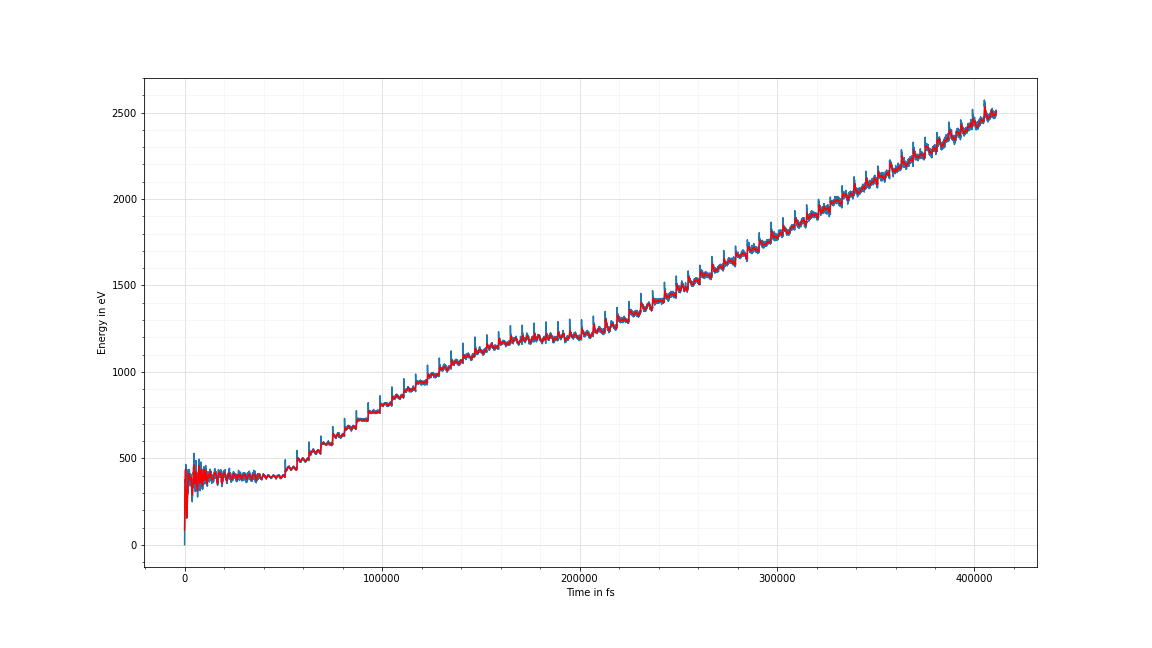
\includegraphics[scale=1]{/home/cm/CLionProjects/MoleDymCode/AData/Clusters/kineticEnergyCurve14.png} 
    \end{center} 
    \caption[Gold Cluster Simulation with 10179 Atoms]{Gold Cluster Simulation with 10179 Atoms} 
    \label{GoldClusterSimulationKineticTime10179} 
\end{figure} 
 
\begin{figure}[!h] 
    \begin{center} 
        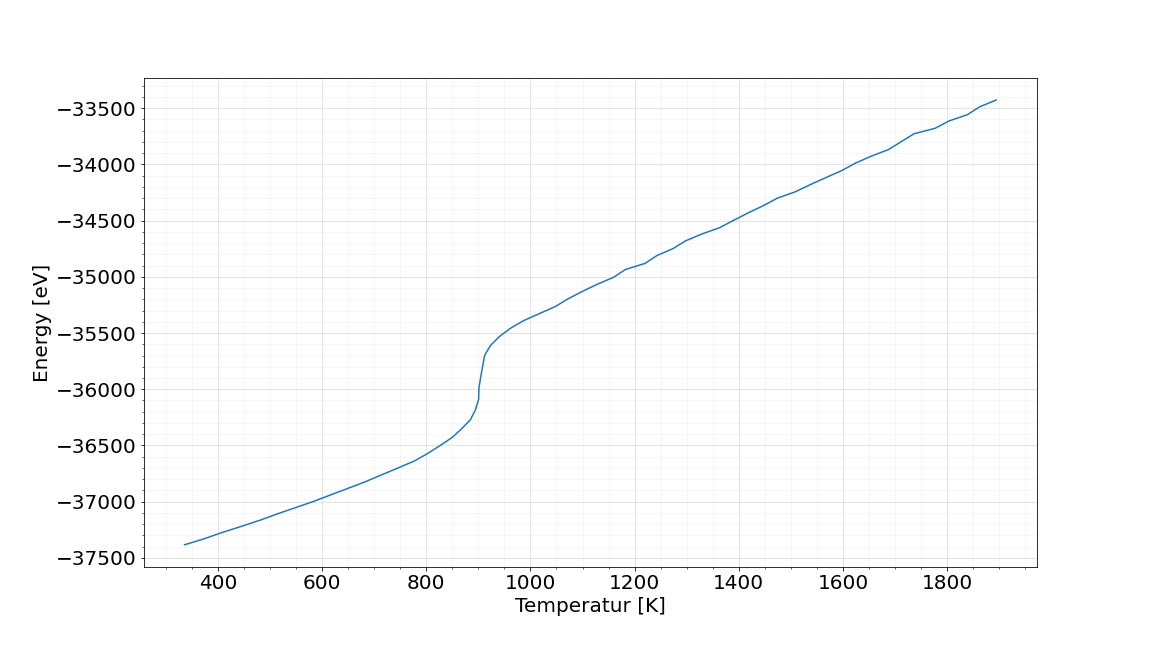
\includegraphics[scale=1]{/home/cm/CLionProjects/MoleDymCode/AData/Clusters/temperaturPotentialEnergyCurve14.png} 
    \end{center} 
    \caption[Gold Cluster Simulation with 10179 Atoms]{Gold Cluster Simulation with 10179 Atoms} 
    \label{GoldClusterSimulationTemperaturEnergy10179} 
\end{figure} 
 
\begin{figure}[!h] 
    \begin{center} 
        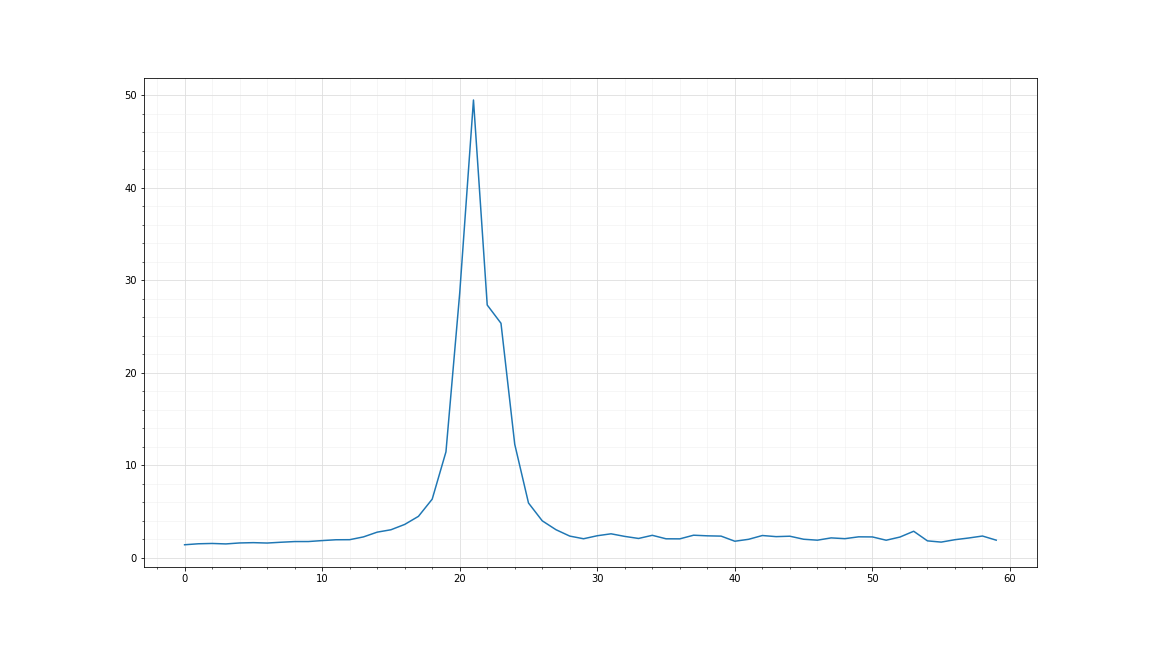
\includegraphics[scale=1]{/home/cm/CLionProjects/MoleDymCode/AData/Clusters/temperaturEnergyCurveGradients14.png} 
    \end{center} 
    \caption[Gradient of Temperatur and Energy for the Gold Cluster Simulation with 10179 Atoms]{Gradient of Temperatur and Energy for the Gold Cluster Simulation with 10179 Atoms} 
    \label{GoldClusterSimulationGradient10179} 
\end{figure} 
 
